\chapter{Lalu Lintas Membran dan Penyortiran Protein}\label{ch:b3:membrane-traffic}

Sebuah sel pankreas membuat sekitar sepuluh juta molekul enzim pencernaan tiap
menit, mengemasnya menjadi butiran, lalu melepaskannya ke dalam sebuah saluran
atas isyarat dari ususnya --- tanpa sekali pun membiarkan satu molekul tripsin
lepas di dalam sitoplasmanya sendiri. Sebuah sel hati mengambil kolesterol dari
darah dengan menelan butiran pengusungnya secara utuh, dengan laju ribuan tiap
menit, lalu mengembalikan tiap reseptornya ke permukaan demi butiran
berikutnya. Sebuah protein yang baru dibuat dan ditujukan ke mitokondria,
nukleus, \omterm{def:b3:membrane-traffic:endocytosis}{lisosom}, membran, atau dunia luar mencapai alamatnya di antara
selusin kompartemen dengan laju galat yang akan memalukan sebuah layanan pos.
Bab ini membahas penyortirannya: isyarat yang tertulis di dalam protein, mesin
yang membacanya, vesikel yang mengusung membran dan muatan antarkompartemen,
\omterm{def:b3:membrane-traffic:coats}{salut} yang membentuk vesikelnya dan protein yang membuatnya berfusi dengan
sasaran yang benar, serta lalu lintas dua arah --- sekresi keluar, endositosis
masuk --- yang dijaga sebuah sel eukariot setiap detik hidupnya.

\section{Isyarat dan alamat}

\begin{definition}[Isyarat penyortiran]\label{def:b3:membrane-traffic:signals}
\index{isyarat penyortiran}\index{peptida isyarat}%
\index{isyarat penempatan nukleus}\index{praurutan}
Sebuah \emph{isyarat penyortiran} adalah segmen sebuah protein, atau sebuah
modifikasinya, yang dibaca sebuah reseptor yang mengantarkan protein itu ke
satu kompartemen. \emph{Peptida isyarat}, yaitu bentangan \numrange{15}{30}
residu pada ujung aminonya dengan inti hidrofob, mengirim sebuah protein ke
dalam retikulum endoplasma selagi protein itu dibuat; dari situ rute bakunya
menuju Golgi lalu ke membran plasma atau ke luar, dan isyarat lanjutan
membelokkannya ke \omterm{def:b3:membrane-traffic:endocytosis}{lisosom} (sebuah gula terfosforilasi) atau kembali ke
retikulumnya (urutan karboksi-terminal KDEL). Sebuah \emph{isyarat penempatan
nukleus}, yaitu tambalan basa yang pendek seperti PKKKRKV, diikat importin
yang mengusung protein terlipat itu melewati pori intinya; sebuah
\emph{praurutan} mitokondria, yaitu heliks amfipatik sepanjang
\numrange{20}{50} residu, dikenali reseptor pada membran luarnya lalu
disusupkan, dalam keadaan tak terlipat, melewati translokase kedua membrannya;
enzim peroksisom berakhir dengan SKL. Protein yang tak memiliki satu pun
isyarat itu tinggal di dalam sitosol. Setiap isyarat ditemukan dengan cara yang
sama: menghapusnya meninggalkan proteinnya di dalam sitosol, mencangkokkannya
pada protein sitosol mengirim protein itu ke kompartemennya.
\end{definition}

\begin{proof}[Bukti eksperimental]
Blobel dan Dobberstein (1975) mentranslasikan RNA duta sebuah rantai ringan
antibodi di dalam sistem bebas sel. Tanpa membran, hasilnya lebih panjang
kira-kira dua puluh residu daripada protein yang disekresikan;
dengan pecahan retikulum endoplasma yang ditambahkan \emph{selama} translasi,
hasilnya berukuran seperti protein sekresinya dan terlindung dari protease
tambahan --- hasilnya berada di dalam vesikel --- sedangkan membran yang
ditambahkan sesudah translasi tidak berbuat apa-apa. Segmen amino-terminal
tambahan itu, yaitu \omterm{def:b3:membrane-traffic:signals}{peptida isyarat}, dibutuhkan untuk masuk ke retikulumnya,
dibuang di dalamnya, dan hanya bekerja selagi rantainya dibuat: itulah
\emph{hipotesis isyarat}, yang terkukuhkan dalam segala rinciannya ketika
reseptornya (partikel pengenal isyarat, Walter dan Blobel 1981) dan salurannya
(Sec61) dimurnikan.
\end{proof}

\begin{omfigure}
\begin{tikzpicture}[every node/.style={font=\scriptsize}, >=stealth]
  % ER membrane
  \fill[omDef!15] (0,0) rectangle (12,-1.6);
  \draw[very thick, omDef] (0,0) -- (12,0); \draw[very thick, omDef] (0,-0.35) -- (12,-0.35);
  \node[right, omDef!70!black] at (0.1,-1.3) {lumen RE};
  \node[right] at (0.1,2.9) {sitosol};
  % stage 1: ribosome with emerging signal peptide + SRP
  \draw[thick, fill=gray!25] (1.4,1.6) circle (0.5); \draw[thick, fill=gray!25] (1.4,0.95) ellipse (0.62 and 0.3);
  \draw[very thick, omThm] (1.4,0.65) -- (1.4,0.2) -- (1.9,0.1);
  \draw[thick, fill=omProp!40] (2.1,0.35) ellipse (0.35 and 0.2); \node[above right] at (2.2,0.5) {SRP};
  \node[below, align=center] at (1.7,-1.7) {1. peptida isyarat muncul;\\SRP mengikat, translasi berhenti sejenak};
  % stage 2: docking at SRP receptor and translocon
  \draw[->, thick] (3.2,1.2) -- (4.2,1.2);
  \draw[thick, fill=gray!25] (5.6,1.75) circle (0.5); \draw[thick, fill=gray!25] (5.6,1.1) ellipse (0.62 and 0.3);
  \draw[thick, fill=omMeth!40] (5.2,0.0) rectangle (5.45,-0.35); \draw[thick, fill=omMeth!40] (5.75,0.0) rectangle (6.0,-0.35);
  \node[below, align=center] at (5.9,-1.7) {2. reseptor SRP melabuhkannya\\pada Sec61; SRP pergi};
  \draw[very thick, omThm] (5.6,0.8) -- (5.6,-0.2);
  \draw[thick, fill=omProp!40] (4.7,0.15) ellipse (0.3 and 0.18); \node[above] at (4.7,0.33) {reseptor SRP};
  % stage 3: translocation, cleavage, glycosylation
  \draw[->, thick] (7.2,1.2) -- (8.2,1.2);
  \draw[thick, fill=gray!25] (9.6,1.75) circle (0.5); \draw[thick, fill=gray!25] (9.6,1.1) ellipse (0.62 and 0.3);
  \draw[thick, fill=omMeth!40] (9.2,0.0) rectangle (9.45,-0.35); \draw[thick, fill=omMeth!40] (9.75,0.0) rectangle (10.0,-0.35);
  \draw[very thick, omThm] (9.6,0.8) -- (9.6,-0.5) .. controls (9.6,-1.0) and (10.3,-1.1) .. (10.6,-0.7);
  \draw[omThm, thick] (10.9,-0.9) -- (11.2,-0.9); \node[right, font=\tiny] at (11.0,-1.15) {isyarat dipotong};
  \fill[omExo] (10.3,-1.0) circle (0.07); \fill[omExo] (10.45,-1.12) circle (0.07); \node[below, font=\tiny] at (10.2,-1.15) {gula};
  \node[below, align=center] at (10.0,-1.7) {3. rantainya menyeberang selagi dibuat;\\isyaratnya dipotong, gulanya ditambahkan};
\end{tikzpicture}

{\small Hipotesis isyarat. Sebuah \omterm{def:b3:membrane-traffic:signals}{peptida isyarat} pada awal rantai
nasennya diikat partikel pengenal isyarat, yang menghentikan translasinya
sejenak lalu melabuhkan ribosomnya pada saluran Sec61; rantainya lalu
menyeberangi membrannya selagi disintesis, isyaratnya dipotong di dalam
lumennya, dan gulanya ditambahkan.}
\end{omfigure}

\begin{proposition}[Protein membran dan topologinya]\label{prop:b3:membrane-traffic:topology}
\index{urutan henti-pindah}\index{topologi membran}
Sebuah bentangan hidrofob sepanjang kira-kira dua puluh residu di tengah
rantai yang sedang ditranslokasikan bertindak sebagai urutan
\emph{henti-pindah}: salurannya membuka ke samping lalu melepaskannya ke dalam
lapis rangkapnya sebagai heliks lintas membran, dengan bagian yang sudah
ditranslokasikan berada di dalam lumennya dan sisanya dibuat ke arah sitosol.
Bentangan kedua semacam itu memulai kembali translokasinya, dan sebuah protein
dengan $n$ isyarat berselang-seling berakhir dengan $n$ heliks yang menembus
membran. Orientasi yang ditetapkan di dalam retikulumnya tak pernah berubah:
apa yang menghadap lumen retikulumnya menghadap lumen Golgi dan lumen setiap
vesikel sesudahnya, dan menghadap \emph{luar} sel sesudah fusi dengan membran
plasmanya. Karena itu gulanya, yang hanya ditambahkan di dalam lumennya, selalu
berada pada muka ekstrasel sebuah protein permukaan, dan topologi sebuah
reseptor dapat dibaca dari tempat tapak glikosilasinya berada.
\end{proposition}

\begin{method}[Denyut--kejar]\label{met:b3:membrane-traffic:pulse-chase}
\index{denyut--kejar}\index{autoradiografi}
Untuk mengikuti sekumpulan molekul yang baru dibuat melewati selnya: (1)
paparkanlah selnya sejenak (yaitu \emph{denyutnya}, beberapa menit) pada
pendahulu yang radioaktif atau bertanda lain --- leusina bertritium bagi
proteinnya; (2) gantilah dengan pendahulu tak berlabel yang berlebih (yaitu
\emph{kejarnya}), sehingga tak ada label baru yang disisipkan; (3) fiksasilah
contoh selnya pada selang waktu tertentu lalu temukan labelnya dengan
autoradiografi pada mikrograf elektron, atau dengan memisahkan kompartemennya
lalu mencacahnya; (4) plotlah bagian label di tiap kompartemennya terhadap
waktu. Urutan pengisian dan pengosongan kompartemennya adalah rutenya;
penataan waktunya memberi waktu tinggal di masing-masing. Laboratorium Palade
(dasawarsa 1960-an) menerapkannya pada sel asinar pankreas dan menemukan
labelnya di dalam retikulum kasar pada \qty{3}{min}, di dalam Golgi pada
\qty{20}{min}, di dalam vakuola pemekat dan butiran pada \qty{40}{min}, dan di
dalam salurannya sesudah sejam dan atas sebuah isyarat: itulah jalur sekresi,
yang terbentang dalam waktu.
\end{method}

\begin{theorem}[Kompartemen berurutan dan kurva denyut--kejarnya]\label{thm:b3:membrane-traffic:pulse-chase}
\index{model kompartemen}
Misalkan sedenyut protein berlabel meninggalkan kompartemen $A$ menuju $B$
dengan laju orde satu $k_{1}$ lalu meninggalkan $B$ menuju $C$ dengan laju
$k_{2}$, dengan $C$ menahannya. Dengan seluruh labelnya di $A$ pada $t = 0$,
\[
A(t) = e^{-k_{1}t},\qquad
B(t) = \frac{k_{1}}{k_{2} - k_{1}}\bigl(e^{-k_{1}t} - e^{-k_{2}t}\bigr),
\qquad
C(t) = 1 - A - B,
\]
dan label di $B$ memuncak pada $t^{*} = \ln(k_{2}/k_{1})/(k_{2} - k_{1})$.
Waktu tinggal rata-rata di $A$ adalah $1/k_{1}$ dan di $B$ adalah $1/k_{2}$,
apa pun urutan kedua lajunya.
\end{theorem}
\begin{proof}
$\mathrm{d}A/\mathrm{d}t = -k_{1}A$ memberi eksponensialnya. Bagi $B$,
$\mathrm{d}B/\mathrm{d}t = k_{1}A - k_{2}B = k_{1}e^{-k_{1}t} - k_{2}B$;
cobalah $B = \beta(e^{-k_{1}t} - e^{-k_{2}t})$: turunannya adalah
$\beta(-k_{1}e^{-k_{1}t} + k_{2}e^{-k_{2}t})$ dan $-k_{2}B = \beta(-k_{2}
e^{-k_{1}t} + k_{2}e^{-k_{2}t})$, sehingga persamaannya menuntut $\beta(k_{2}
- k_{1})e^{-k_{1}t} = k_{1}e^{-k_{1}t}$, $\beta = k_{1}/(k_{2} -
k_{1})$, dan $B(0) = 0$ seperti yang dituntut. Dengan menetapkan $\mathrm{d}B/\mathrm{d}t =
0$: $k_{1}e^{-k_{1}t} = k_{2}e^{-k_{2}t}$, sehingga diperoleh $t^{*}$. Waktu
rata-rata sebuah molekul tinggal di kompartemen yang ditinggalkannya dengan
laju $k$ adalah $\int_{0}^{
\infty} t\,k e^{-kt}\,\mathrm{d}t = 1/k$.
\end{proof}

\begin{example}[Sel Palade dalam angka]\label{ex:b3:membrane-traffic:palade}
Ambillah $k_{1} = \qty{0.1}{min^{-1}}$ (sepuluh menit di dalam retikulumnya)
dan $k_{2} = \qty{0.05}{min^{-1}}$ (dua puluh menit di dalam Golginya).
Golginya memuncak pada $t^{*} = \ln 2/0.05 = \qty{13.9}{min}$, dan ketika itu
menahan $B = 2(e^{-1.39} -
e^{-0.69}) = 2(0.25 - 0.50)\cdot(-1) = 0.50$: separuh labelnya. Pada
\qty{40}{min}, $A = 0.018$, $B = 2(0.018 - 0.135) \to 0.23$, $C = 0.75$:
tiga perempat proteinnya telah mencapai butirannya. Kurva yang teramati di
laboratorium Palade berbentuk seperti itu, dan mencocokkannya adalah cara
waktu tinggalnya pertama kali diukur.
\end{example}

\begin{omfigure}
\begin{tikzpicture}
\begin{axis}[
  width=0.7\linewidth, height=5.6cm,
  axis x line=bottom, axis y line=left,
  xmin=0, xmax=80, ymin=0, ymax=1.05,
  xlabel={menit sesudah denyutnya}, ylabel={bagian labelnya},
  xlabel style={font=\small, at={(axis description cs:0.5,-0.12)}, anchor=north},
  ylabel style={font=\small},
  tick label style={font=\small}, xtick={0,20,40,60,80}, ytick={0,0.5,1},
  clip=false,
]
\addplot[very thick, omDef, domain=0:80, samples=80] {exp(-0.1*x)};
\addplot[very thick, omProp, domain=0:80, samples=80] {2*(exp(-0.05*x)-exp(-0.1*x))};
\addplot[very thick, omMeth!70!black, domain=0:80, samples=80] {1-exp(-0.1*x)-2*(exp(-0.05*x)-exp(-0.1*x))};
\node[font=\scriptsize, omDef, anchor=south west] at (axis cs:4,0.62) {retikulum, $A$};
\node[font=\scriptsize, omProp, anchor=south] at (axis cs:14,0.53) {Golgi, $B$};
\node[font=\scriptsize, omMeth!70!black, anchor=north west] at (axis cs:45,0.72) {butiran, $C$};
\end{axis}
\end{tikzpicture}

{\small Kurva denyut--kejar dari model dua laju dengan $k_{1} =
\qty{0.1}{min^{-1}}$ dan $k_{2} = \qty{0.05}{min^{-1}}$: labelnya meninggalkan
retikulumnya secara eksponensial, melewati Golginya dengan puncak pada
\qty{14}{min}, lalu menumpuk di dalam butirannya.}
\end{omfigure}

\section{Retikulum endoplasma: pelipatan, gula, dan mutu}

\begin{definition}[N-glikosilasi dan kendali mutu]\label{def:b3:membrane-traffic:glycosylation}
\index{N-glikosilasi}\index{daur kalneksin}%
\index{penguraian terkait RE}\index{tanggapan protein tak terlipat}
Begitu rantainya masuk ke lumennya, sebuah oligosakarida berisi empat belas
gula yang telah dirakit lebih dahulu (dua N-asetilglukosamina, sembilan
manosa, tiga glukosa) dipindahkan dari pengusung lipid ke asparagina di dalam
urutan Asn-X-Ser/Thr --- itulah \emph{N-glikosilasi}. Ketiga glukosanya lalu
dipangkas satu demi satu, dan pemangkasannya menjadi jam pelipatan: protein
yang masih mengusung satu glukosa ditahan \omterm{def:b3:structural-biology:chaperones}{pendamping} bernama kalneksin;
protein yang glukosa terakhirnya telah dibuang tetapi belum terlipat
diglukosilasi ulang oleh enzim yang mengenali tambalan hidrofob yang terpapar,
lalu kembali ke kalneksin --- itulah \emph{daur kalneksin}. Protein yang gagal
berulang kali ditarik kembali ke dalam sitosol, diubikuitinasi, lalu
dimusnahkan proteasom: itulah \emph{penguraian terkait RE}
(ERAD). Ketika protein tak terlipat menumpuk lebih cepat daripada yang dapat
dilipat atau dimusnahkan, pengindera pada membran retikulumnya melancarkan
\emph{tanggapan protein tak terlipat}: translasinya diperlambat, gen
\omterm{def:b3:structural-biology:chaperones}{pendampingnya} diimbas, retikulumnya diperluas, dan, bila cekamannya bertahan,
selnya dibunuh. Mutasi fibrosis kistik yang paling lazim
($\Delta$F508 pada CFTR) membuat sebuah saluran yang sebenarnya akan bekerja
tetapi terlalu lambat melipat, tertangkap ERAD, dan tak pernah mencapai
permukaannya; obat yang membantunya melipat kini menjadi pengobatan.
\end{definition}

\begin{omfigure}
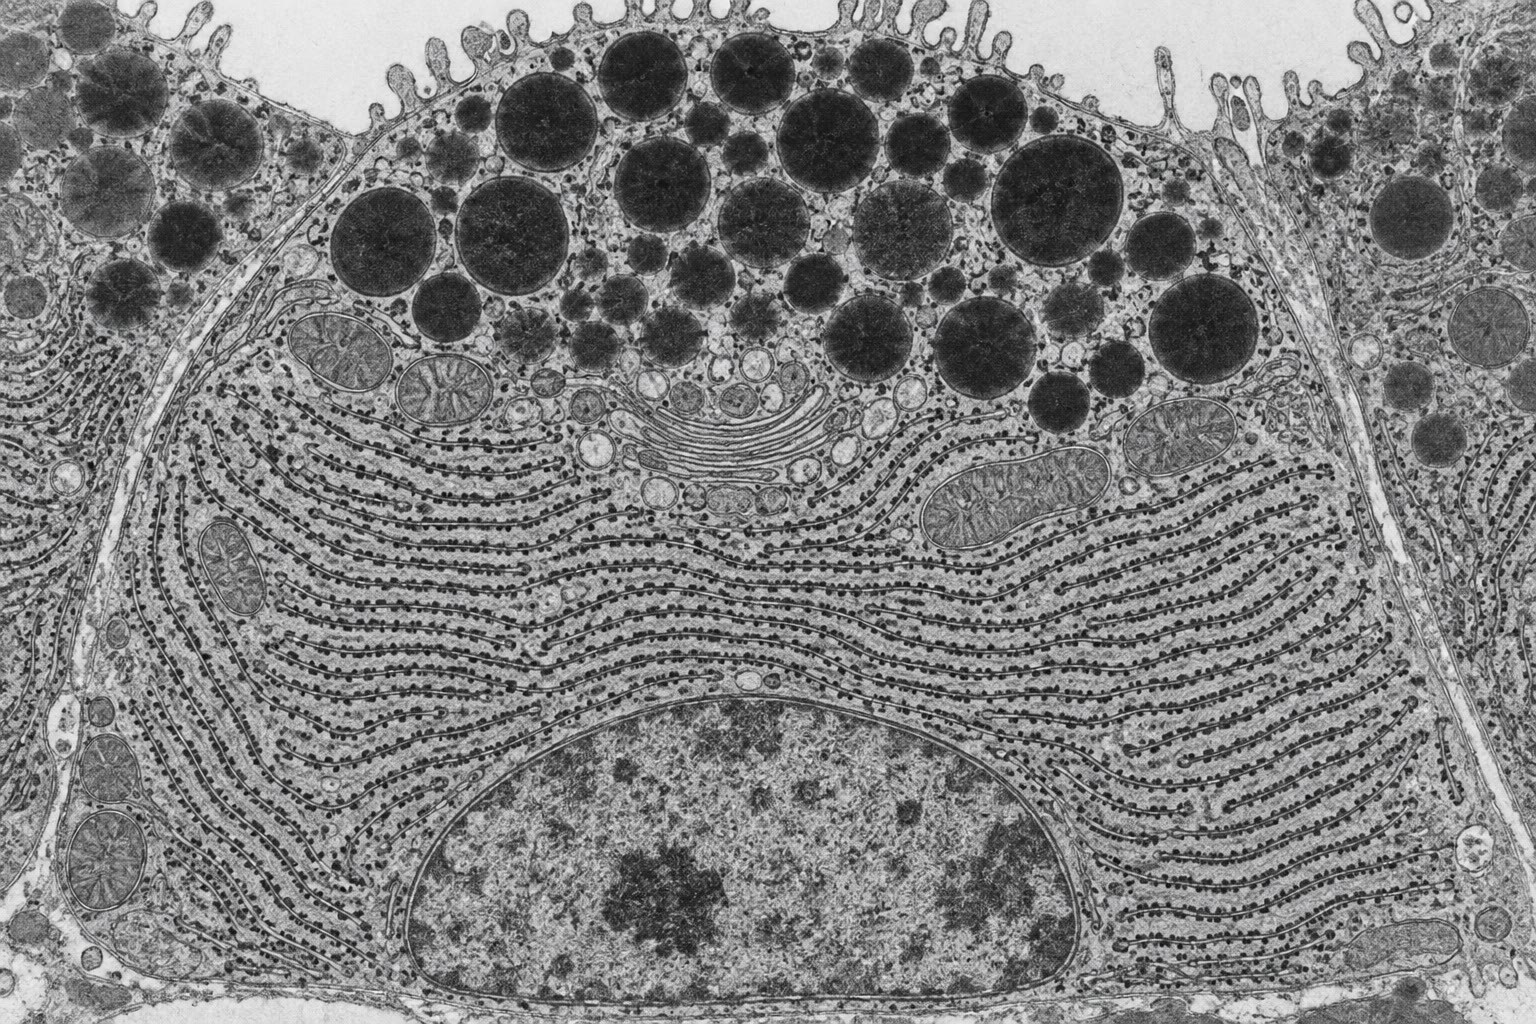
\includegraphics[width=0.56\linewidth]{images/book5/ai/b5-08-pancreas-acinar.jpg}

{\small Sebuah sel asinar pankreas di bawah mikroskop elektron: retikulum
endoplasma kasar yang bertumpuk dan bertaburan ribosom memenuhi bagian
dasarnya, Golginya terletak di atas nukleusnya, dan butiran sekresi yang padat
berisi enzim pencernaan terkemas di bawah permukaan apikalnya, menunggu sebuah
isyarat.}
\end{omfigure}

\section{Vesikel: pertunasan, penyasaran, fusi}

\begin{definition}[Salut dan pertunasan vesikel]\label{def:b3:membrane-traffic:coats}
\index{vesikel bersalut}\index{COPII}\index{COPI}\index{klatrin}\index{GTPase kecil}
Sebuah vesikel angkutan dibentuk oleh \emph{salut} protein yang dirakit pada
muka sitosol sebuah membran, yang melengkungkan membrannya menjadi tunas
sebesar \qtyrange{60}{100}{nm}, mengumpulkan muatannya lewat reseptor yang
menembus membrannya, lalu dilepaskan sesudah vesikelnya mencuwil. Tiga salut
melayani rute utamanya: \emph{COPII} bagi vesikel yang meninggalkan
retikulumnya menuju Golgi, \emph{COPI} bagi lalu lintas balik dari Golgi ke
retikulumnya dan antarsisterna Golgi, serta \emph{klatrin} --- protein
berkaki tiga yang berpolimerisasi menjadi sangkar heksagon dan pentagon ---
bagi vesikel yang meninggalkan trans-Golgi menuju \omterm{def:b3:membrane-traffic:endocytosis}{endosom} dan bagi
endositosis pada membran plasma, dan di situ protein adaptor menghubungkan
sangkarnya dengan reseptor yang sedang diinternalisasi. Tiap salut direkrut
sebuah \emph{GTPase kecil} (Sar1 bagi COPII, Arf1 bagi COPI dan klatrin) yang
menyisip ke dalam membrannya dalam bentuk GTP-nya dan, begitu menghidrolisis
GTP sesudah pertunasan, membiarkan salutnya luruh. Isyarat pengambilan kembali
menjaga kompartemennya tetap berbeda: protein retikulum yang lolos dan
mengusung KDEL diikat sebuah reseptor di dalam Golgi lalu dibawa kembali di
dalam vesikel COPI.
\end{definition}

\begin{omfigure}
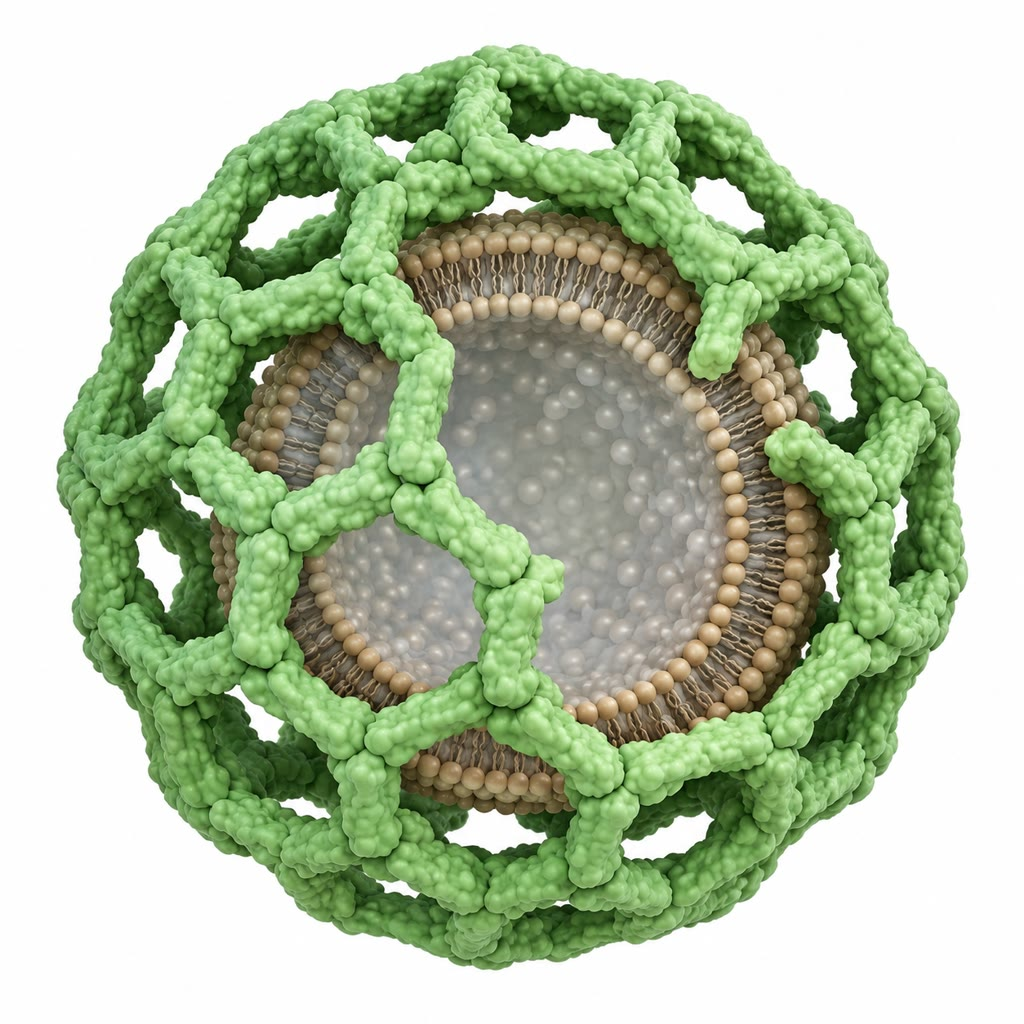
\includegraphics[width=0.36\linewidth]{images/book5/ai/b5-08-clathrin-cage.jpg}\hspace{0.04\linewidth}
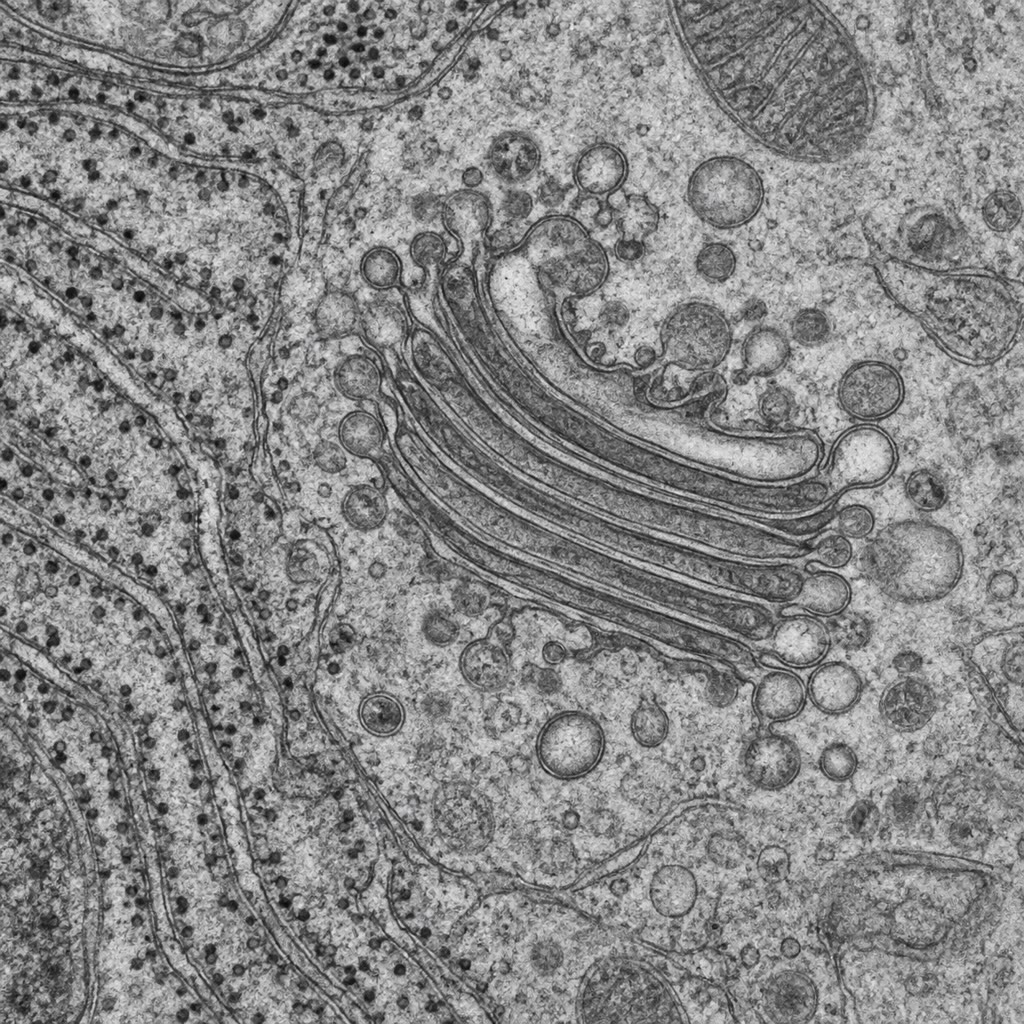
\includegraphics[width=0.36\linewidth]{images/book5/ai/b5-08-golgi-tem.jpg}

{\small Kiri: sebuah sangkar \omterm{def:b3:membrane-traffic:coats}{klatrin}, yaitu kisi polihedral berisi satuan
berkaki tiga yang membentuk sebuah vesikel endositik (dipotong agar membrannya
di dalam terlihat). Kanan: sebuah tumpukan Golgi di bawah mikroskop elektron,
yaitu setumpuk sisterna gepeng dengan vesikel yang bertunas dari tepinya.}
\end{omfigure}

\begin{definition}[Penyasaran dan fusi]\label{def:b3:membrane-traffic:fusion}
\index{GTPase Rab}\index{SNARE}\index{fusi membran}\index{sinaptotagmin}
Sebuah vesikel menemukan sasarannya lewat dua lapis pengenalan. \emph{GTPase
Rab} --- sekitar enam puluh di dalam sel manusia, masing-masing pada membran
satu kompartemen --- merekrut protein penambat yang panjang yang menangkap
vesikel datang yang mengusung Rab yang cocok. Lalu \emph{SNARE} bekerja: sebuah
v-SNARE pada vesikelnya dan t-SNARE pada sasarannya, yakni protein heliks yang
tertambat pada membrannya masing-masing, melilit satu sama lain dari ujung
jauhnya ke arah membrannya, dan energi berkas empat heliks yang terbentuk itu
menarik kedua lapis rangkapnya sampai berfusi. Tiap pasangan SNARE bersifat
khas, yakni pemeriksaan kedua atas alamatnya. Sesudah fusinya, berkasnya
dicungkil terpisah oleh ATPase bernama NSF agar dapat dipakai lagi. Fusinya
dapat dibuat menunggu sebuah isyarat: di dalam terminal saraf, SNARE-nya
ditahan setengah terkancing oleh kompleksin sampai \emph{sinaptotagmin}, yang
mengikat kalsium yang masuk ketika sebuah potensial aksi tiba, menuntaskan
pengancingannya dalam kurang dari satu milidetik --- yakni pelepasan
neurotransmiter yang dibahas pada jilid Tahun~2. Neurotoksin tetanus dan
botulisme adalah protease yang memotong SNARE.
\end{definition}

\begin{proof}[Bukti eksperimental]
Novick dan Schekman (1980) memisahkan mutan khamir yang peka suhu
yang berhenti menyekresi pada \qty{37}{\celsius} lalu menimbun
proteinnya di kompartemen mana pun yang terhalang cacatnya --- retikulum,
Golgi, atau vesikel yang menumpuk di bawah permukaannya; ke-$23$ gen \emph{sec}
itu menetapkan langkahnya dan, begitu diklon, ternyata menyandikan \omterm{def:b3:membrane-traffic:coats}{salutnya},
GTPase-nya, serta \omterm{def:b3:membrane-traffic:fusion}{SNARE-nya}. Rothman menyusun ulang angkutan antarsisterna
Golgi di dalam tabung reaksi dengan membran, sitosol, dan ATP yang telah
dimurnikan, lalu dari situ memurnikan NSF dan \omterm{def:b3:membrane-traffic:fusion}{SNARE-nya}; kedua pendekatan itu
memusat pada protein yang sama, dan mesin khamir serta mesin mamalianya
ternyata sama.
\end{proof}

\begin{omfigure}
\begin{tikzpicture}[every node/.style={font=\scriptsize}, >=stealth]
  % three stages left to right
  \foreach \x/\gap/\lab in {0/1.2/{1. ditambat Rab}, 4.4/0.55/{2. SNARE terkancing}, 8.8/0.0/{3. fusi, muatan dilepaskan}} {
    % target membrane
    \draw[very thick, omDef] (\x,0) -- (\x+3.4,0); \draw[very thick, omDef] (\x,-0.3) -- (\x+3.4,-0.3);
    \node[below, align=center] at (\x+1.7,-0.45) {\lab};
  }
  % stage 1 vesicle
  \draw[very thick, omProp] (1.7,1.2+0.8) circle (0.8); \draw[very thick, omProp] (1.7,1.2+0.8) circle (0.6);
  \draw[omThm, thick] (1.4,1.25) -- (1.4,0.35); \draw[omThm, thick] (2.0,1.25) -- (2.0,0.35);
  \draw[omMeth!70!black, thick] (1.7,1.2) -- (1.7,0.6); \draw[omMeth!70!black, thick] (1.7,0.6) -- (1.7,0.0);
  \draw[thick, fill=omExo!40] (0.7,0.9) ellipse (0.25 and 0.2); \node[left] at (0.45,0.9) {Rab};
  \draw[thick, omExo!70!black] (0.95,0.9) .. controls (1.1,0.5) .. (1.2,0.05); \node[left, font=\tiny] at (0.9,0.4) {penambat};
  \node[right, font=\tiny] at (2.05,0.8) {SNARE};
  % stage 2 vesicle closer, helices twisted
  \draw[very thick, omProp] (6.1,0.55+0.8) circle (0.8); \draw[very thick, omProp] (6.1,0.55+0.8) circle (0.6);
  \draw[omThm, very thick] (5.85,0.6) .. controls (6.2,0.5) and (5.9,0.3) .. (6.1,0.05);
  \draw[omMeth!70!black, very thick] (6.35,0.6) .. controls (6.0,0.5) and (6.3,0.3) .. (6.1,0.05);
  \node[right, font=\tiny, align=left] at (6.6,0.35) {berkas empat heliks\\menarik membrannya\\bersatu};
  % stage 3 fused omega shape
  \draw[very thick, omProp] (9.7,0) .. controls (9.7,1.5) and (11.3,1.5) .. (11.3,0);
  \draw[very thick, omProp] (9.9,-0.3) .. controls (9.9,1.1) and (11.1,1.1) .. (11.1,-0.3);
  \foreach \p in {(10.5,-0.9),(10.2,-1.1),(10.8,-1.15)} \fill[omExo] \p circle (0.06);
  \draw[->, omExo, thick] (10.5,0.5) -- (10.5,-0.6);
  \node[right, font=\tiny, align=left] at (11.4,0.8) {NSF kemudian\\membuka kancing\\SNARE-nya};
\end{tikzpicture}

{\small Fusi dalam tiga langkah. Sebuah Rab pada vesikelnya dan sebuah
penambat pada sasarannya membawa kedua membrannya ke dalam jangkauan; \omterm{def:b3:membrane-traffic:fusion}{SNARE}
vesikel dan \omterm{def:b3:membrane-traffic:fusion}{SNARE} sasarannya (merah dan hijau) terkancing menjadi berkas empat
heliks yang menyeret kedua lapis rangkapnya bersatu; keduanya berfusi dan
muatannya masuk ke kompartemen sasarannya.}
\end{omfigure}

\begin{proposition}[Golgi]\label{prop:b3:membrane-traffic:golgi}
\index{aparatus Golgi}\index{pematangan sisterna}\index{manosa-6-fosfat}
Golgi adalah tumpukan empat sampai delapan sisterna gepeng, dengan muka cis
menghadap retikulumnya dan muka trans menghadap membran plasmanya, dan tiap
sisternanya memuat perangkat enzim yang berlainan yang memangkas dan membangun
ulang gula glikoprotein yang lewat serta menambahkan gula berpaut-O, sulfat,
dan fosfat. Muatannya melaju terutama lewat \emph{\omterm{prop:b3:membrane-traffic:golgi}{pematangan sisterna}}: sebuah
sisterna baru terbentuk pada muka cisnya dari vesikel yang datang, bergerak
melewati tumpukannya sebagaimana sisterna sebelumnya, lalu matang seiring
vesikel \omterm{def:b3:membrane-traffic:coats}{COPI} mengusung enzim tiap sisterna mundur ke sisterna yang lebih muda
di belakangnya; pada muka transnya sisterna itu pecah menjadi vesikel yang
menuju tujuannya. Di situlah penyortirannya diputuskan: hidrolase \omterm{def:b3:membrane-traffic:endocytosis}{lisosom}, yang
ditandai di dalam Golgi cis dengan \emph{manosa-6-fosfat}, diikat reseptornya
lalu dikemas ke dalam vesikel \omterm{def:b3:membrane-traffic:coats}{klatrin} menuju \omterm{def:b3:membrane-traffic:endocytosis}{endosom}; protein sekresi yang
teratur menggumpal pada pH yang agak asam menjadi butiran pemekat; selebihnya
pergi lewat arus konstitutif menuju permukaannya. Pada penyakit sel-I, enzim
pemfosforilasinya tak ada, hidrolasenya disekresikan alih-alih diantarkan, dan
\omterm{def:b3:membrane-traffic:endocytosis}{lisosomnya} terisi bahan yang tak tercerna.
\end{proposition}

\begin{omfigure}
\begin{tikzpicture}[every node/.style={font=\scriptsize}, >=stealth]
  % plasma membrane top
  \draw[very thick, omDef] (0,4.2) -- (12,4.2); \node[above] at (6,4.25) {membran plasma \quad (luar di atas)};
  % ER
  \draw[thick, fill=omDef!12] (0.3,0.0) rectangle (4.0,0.9); \node at (2.15,0.45) {retikulum endoplasma};
  % Golgi stack
  \foreach \y in {1.5,1.85,2.2,2.55} \draw[thick, fill=omProp!25] (4.8,\y) ellipse (1.4 and 0.13);
  \node[right] at (6.3,1.5) {cis}; \node[left] at (3.35,2.55) {trans};
  \node[right] at (6.3,2.05) {tumpukan Golgi};
  % ER -> Golgi (COPII)
  \draw[->, thick, omMeth!70!black] (3.9,0.95) -- (4.5,1.4); \node[right, omMeth!70!black, font=\tiny] at (4.35,1.02) {COPII};
  % Golgi -> ER (COPI)
  \draw[->, thick, omThm] (3.6,1.42) -- (2.9,0.95); \node[left, omThm, font=\tiny] at (2.95,1.3) {COPI, pengambilan KDEL};
  % trans Golgi -> PM constitutive
  \draw[->, thick, omMeth!70!black] (5.6,2.7) -- (7.6,4.1); \node[left, font=\tiny, align=right] at (6.4,3.6) {sekresi\\konstitutif};
  % trans -> secretory granule -> PM regulated
  \draw[->, thick, omMeth!70!black] (4.6,2.7) -- (4.0,3.3); \draw[thick, fill=omExo!50] (3.8,3.5) circle (0.22); \draw[->, thick, omMeth!70!black] (3.8,3.75) -- (3.8,4.1);
  \node[left, font=\tiny, align=right] at (3.55,3.5) {butiran sekresi:\\teratur, atas isyarat};
  % trans -> endosome/lysosome (clathrin, M6P)
  \draw[->, thick, omProp!80!black] (6.0,2.62) -- (8.25,2.62); \node[above, font=\tiny] at (7.1,2.67) {klatrin, reseptor M6P};
  \draw[thick, fill=omProp!20] (8.8,2.7) circle (0.5); \node at (8.8,2.7) {\tiny endosom};
  \draw[->, thick, omProp!80!black] (9.25,2.4) -- (10.2,1.95); \draw[thick, fill=omThm!25] (10.7,1.6) circle (0.5); \node at (10.7,1.6) {\tiny lisosom};
  % endocytosis from PM to endosome
  \draw[->, thick, omDef] (9.6,4.15) -- (9.1,3.2); \node[right, font=\tiny, align=left] at (9.5,3.7) {endositosis\\(lubang klatrin)};
  % recycling endosome -> PM
  \draw[->, thick, omDef] (8.5,3.2) -- (8.0,4.15); \node[left, font=\tiny] at (8.3,3.3) {daur ulang};
  % lysosome inputs autophagy
  \draw[->, thick, gray] (11.9,0.6) -- (11.1,1.3); \node[below, font=\tiny, align=center] at (11.9,0.55) {autofagosom\\(sitoplasma, organel)};
\end{tikzpicture}

{\small Peta lalu lintas membran. Ke luar (hijau): retikulum ke Golgi di
dalam vesikel \omterm{def:b3:membrane-traffic:coats}{COPII}, Golgi ke permukaan entah secara konstitutif entah lewat
butiran yang menunggu sebuah isyarat. Ke belakang (merah): vesikel \omterm{def:b3:membrane-traffic:coats}{COPI}
mengembalikan protein retikulum yang lolos. Ke bawah (jingga): enzim \omterm{def:b3:membrane-traffic:endocytosis}{lisosom}
yang ditandai manosa-6-fosfat menuju \omterm{def:b3:membrane-traffic:endocytosis}{endosom} dan \omterm{def:b3:membrane-traffic:endocytosis}{lisosom}. Ke dalam (biru):
endositosis dari permukaannya, dengan sebagian besar reseptornya didaur ulang.}
\end{omfigure}

\section{Endositosis dan lisosom}

\begin{definition}[Endositosis]\label{def:b3:membrane-traffic:endocytosis}
\index{endositosis diperantarai reseptor}\index{endosom}\index{lisosom}\index{autofagi}
\emph{Endositosis diperantarai reseptor} memekatkan sebuah ligan yang terikat
pada reseptor permukaan ke dalam lubang bersalut \omterm{def:b3:membrane-traffic:coats}{klatrin}, yang lalu mencuwil
(GTPase bernama dinamin menjepit lehernya) sebagai vesikel sebesar
\qty{100}{nm} --- seribu tiap menit di dalam sebuah fibroblas, sehingga
seluruh membran permukaannya berganti dalam sejam. Vesikelnya berfusi menjadi
\emph{endosom dini}, yang lumennya diasamkan sampai pH~6 oleh sebuah pompa
proton; sebagian besar ligannya melepaskan reseptornya di situ, reseptornya
kembali ke permukaan di dalam vesikel daur ulang, dan ligannya melanjut
seiring endosomnya matang menjadi endosom lanjut (pH~5.5) lalu berfusi dengan
sebuah \emph{lisosom}: sebuah kompartemen pada pH 4.5--5 yang memuat sekitar
enam puluh hidrolase --- protease, nuklease, lipase, glikosidase --- yang
hanya aktif pada pH itu, sehingga rembesan ke dalam sitosol yang netral
sedikit saja merugikan. Lisosomnya juga mencerna bahan milik selnya sendiri
yang diantarkan \emph{autofagi}: sebuah membran rangkap tumbuh mengelilingi
sebagian sitoplasma atau organel yang aus, menutup menjadi sebuah autofagosom,
lalu berfusi dengan lisosomnya; hasilnya dikembalikan ke sitosol. Autofagi
diimbas kelaparan (ia mendaur ulang zat milik selnya sendiri demi energi) dan
membersihkan gumpalan serta mitokondria yang rusak; kegagalannya dikaitkan
dengan kemunduran saraf.
\end{definition}

\begin{proof}[Bukti eksperimental]
Brown dan Goldstein (dasawarsa 1970-an) mengikuti lipoprotein berkerapatan
rendah (LDL), yaitu butiran pengusung kolesterol di dalam darah, ke dalam
fibroblas biakan. LDL-nya terikat secara jenuh pada sekitar \num{20000} tapak
permukaan tiap sel, diinternalisasi dalam hitungan menit ke dalam lubang
bersalut, dan kolesterolnya dilepaskan di dalam \omterm{def:b3:membrane-traffic:endocytosis}{lisosom} lalu mematikan
sintesis kolesterol sel itu sendiri. Fibroblas dari pasien hiperkolesterolemia
turunan tidak mengikat LDL (reseptornya tak ada) atau mengikatnya tetapi
tidak menginternalisasinya (sebuah mutasi pada ekor sitosol reseptornya yang
mencegah penangkapannya oleh adaptor \omterm{def:b3:membrane-traffic:coats}{klatrin}): penyakitnya adalah
cacat endositosis, ekor reseptornya memuat isyarat internalisasi, dan
reseptor yang didaur ulang --- yang masing-masing menempuh ratusan
perjalanan bolak-balik --- tegak sebagai mekanisme umum penyerapannya.
\end{proof}

\begin{proposition}[Penyerapan lewat reseptor yang didaur ulang]\label{prop:b3:membrane-traffic:uptake}
\index{daur ulang reseptor}
Misalkan sebuah sel memiliki $R$ reseptor seluruhnya, dan $S$ di antaranya
berada di permukaan sedangkan $R - S$ berada di dalam dalam perjalanan
kembalinya. Sebuah reseptor permukaan terisi dengan peluang
$\theta = [L]/(K_{d} + [L])$, reseptor yang terisi diinternalisasi dengan laju
$k_{i}$, dan reseptor yang terinternalisasi kembali dengan laju $k_{r}$. Pada
keadaan tunak, fluks ligan ke dalam selnya adalah
\[
J = \frac{R\,k_{i}k_{r}\,\theta}{k_{r} + k_{i}\theta},
\]
yang menjenuh, seiring naiknya kepekatan ligannya, pada $J_{\max} =
R\,k_{i}k_{r}/(k_{i} + k_{r})$: penyerapan sebuah sel dibatasi bukan oleh
reseptornya saja melainkan oleh secepat apa ia dapat membawanya kembali.
\end{proposition}
\begin{proof}
Reseptor permukaannya hilang dengan laju $k_{i}\theta S$ dan diperoleh kembali
dengan laju $k_{r}(R - S)$; pada keadaan tunak keduanya berimbang, sehingga
$S = R\,k_{r}/(k_{r}
+ k_{i}\theta)$. Tiap internalisasi mengusung satu ligan, sehingga $J =
k_{i}\theta S$, yang memberi rumusnya. Ketika $\theta \to 1$ fluksnya
menuju $R\,k_{i}k_{r}/(k_{r} + k_{i})$ --- reseptornya berdaur secepat yang
diizinkan kedua lajunya, dengan bagian $k_{r}/(k_{i} + k_{r})$ di antaranya
berada di permukaan pada tiap saat.
\end{proof}

\begin{example}[Kolesterol butir demi butir]\label{ex:b3:membrane-traffic:ldl}
Sebuah fibroblas dengan $R = \num{20000}$ reseptor LDL, waktu internalisasi
\qty{5}{min} ($k_{i} = \qty{0.2}{min^{-1}}$) dan waktu kembali
\qty{10}{min} ($k_{r} = \qty{0.1}{min^{-1}}$) menyerap, pada LDL yang
menjenuhkan, sebesar $J_{\max} = \num{20000}\times 0.2\times 0.1/0.3 \approx 1300$
butir tiap menit, dengan sepertiga reseptornya berada di permukaan pada tiap
saat; tiap butirnya membawa sekitar \num{1500} molekul
kolesterol, yakni dua juta tiap menit, cukup untuk membangun kira-kira
sepersepuluh mikrometer persegi membran. Seorang heterozigot bagi
hiperkolesterolemia turunan, yang reseptornya separuh, menyerap separuhnya;
kolesterol darahnya berlipat dua, dan penyakit jantungnya datang dua puluh
tahun lebih awal. Statin menaikkan $R$ dengan melaparkan sel hatinya akan
kolesterolnya sendiri.
\end{example}

\begin{omfigure}
\begin{tikzpicture}
\begin{axis}[
  width=0.7\linewidth, height=5.4cm,
  axis x line=bottom, axis y line=left,
  xmin=0, xmax=10, ymin=0, ymax=1500,
  xlabel={kepekatan LDL, $[L]/K_{d}$}, ylabel={butir tiap menit},
  xlabel style={font=\small, at={(axis description cs:0.5,-0.12)}, anchor=north},
  ylabel style={font=\small},
  tick label style={font=\small}, xtick={0,2,4,6,8,10}, ytick={0,500,1000,1333}, yticklabels={0,500,1000,$J_{\max}$},
  clip=false,
]
\addplot[very thick, omDef, domain=0:10, samples=60] {20000*0.2*0.1*(x/(1+x))/(0.1+0.2*(x/(1+x)))};
\addplot[very thick, omThm, domain=0:10, samples=60] {10000*0.2*0.1*(x/(1+x))/(0.1+0.2*(x/(1+x)))};
\addplot[dashed, gray, domain=0:10, samples=2] {1333};
\node[font=\scriptsize, omDef, anchor=north west] at (axis cs:4,900) {$R = \num{20000}$};
\node[font=\scriptsize, omThm, anchor=north west] at (axis cs:4,560) {$R = \num{10000}$ (heterozigot)};
\end{axis}
\end{tikzpicture}

{\small Penyerapan LDL lewat reseptor yang didaur ulang, dari rumus
proposisinya dengan $k_{i} = \qty{0.2}{min^{-1}}$ dan $k_{r} =
\qty{0.1}{min^{-1}}$: menjenuh dengan ligannya, dan menjadi separuh ketika
separuh reseptornya tak ada.}
\end{omfigure}

\begin{remark}[Satu membran, banyak kompartemen]\label{rem:b3:membrane-traffic:one-membrane}
Setiap membran sistem sekresi dan endositiknya, secara topologi, adalah satu
membran: lumen retikulumnya bersinambung, lewat vesikelnya, dengan bagian luar
selnya, dan sebuah lipid atau protein yang dibuat di dalam retikulumnya dapat
mencapai permukaannya tanpa sekali pun menyeberangi sebuah lapis rangkap.
Yang menjaga kompartemennya tetap berbeda bukanlah dinding melainkan lalu
lintasnya --- pengemasan terpilih ke luar, pengambilan terpilih ke belakang,
dan sepasang molekul pengenal yang khas pada tiap fusinya. Kompartemennya
adalah keadaan tunak sebuah aliran, seperti lubuk sebuah sungai, dan sel yang
berhenti berlalu lintas kehilangan geografinya dalam hitungan jam.
\end{remark}

\section{Latihan}

\begin{exercise}[$\star$]\label{exo:b3:membrane-traffic:1}
Berikanlah isyarat dan tujuannya bagi masing-masing: bentangan dua puluh
residu hidrofob pada ujung aminonya; PKKKRKV; sebuah heliks amfipatik
amino-terminal; KDEL pada ujung karboksinya; sebuah
manosa-6-fosfat pada gulanya.
\end{exercise}

\begin{exercise}[$\star$]\label{exo:b3:membrane-traffic:2}
Uraikanlah ketiga pengamatan kunci percobaan Blobel--Dobberstein
dan apa yang ditunjukkan masing-masing.
\end{exercise}

\begin{exercise}[$\star$]\label{exo:b3:membrane-traffic:3}
Sebutkanlah \omterm{def:b3:membrane-traffic:coats}{salut} dan arah angkutannya bagi: retikulum ke Golgi;
Golgi ke retikulum; trans-Golgi ke \omterm{def:b3:membrane-traffic:endocytosis}{endosom}; membran plasma ke
\omterm{def:b3:membrane-traffic:endocytosis}{endosom}.
\end{exercise}

\begin{exercise}[$\star$]\label{exo:b3:membrane-traffic:4}
Mengapa gula sebuah protein membran plasma selalu berada di bagian luar
selnya?
\end{exercise}

\begin{exercise}[$\star\star$]\label{exo:b3:membrane-traffic:5}
Di dalam model \cref{thm:b3:membrane-traffic:pulse-chase} dengan $k_{1}
= \qty{0.2}{min^{-1}}$ dan $k_{2} = \qty{0.05}{min^{-1}}$, carilah kapan
label Golginya memuncak dan berapa banyak yang ada di sana pada puncaknya;
lalu bagian yang berada di dalam butirannya pada \qty{60}{min}.
\end{exercise}

\begin{exercise}[$\star\star$]\label{exo:b3:membrane-traffic:6}
Sebuah protein membran memiliki bentangan hidrofob sepanjang $22$ residu pada
kedudukan 30, 90, 150, dan 210 serta sebuah \omterm{def:b3:membrane-traffic:signals}{peptida isyarat} amino-terminal.
Gambarkanlah atau uraikanlah topologinya: berapa heliksnya, dan tiap segmen di
antaranya menghadap sisi yang mana. Di mana ia dapat diglikosilasi?
\end{exercise}

\begin{exercise}[$\star\star$]\label{exo:b3:membrane-traffic:7}
Dengan \cref{prop:b3:membrane-traffic:uptake} dan $R = \num{30000}$,
$k_{i} = \qty{0.25}{min^{-1}}$, $k_{r} = \qty{0.05}{min^{-1}}$, hitunglah
$J_{\max}$ dan bagian reseptor yang berada di permukaan pada kejenuhan.
Perubahan tunggal apa yang akan melipatduakan penyerapannya?
\end{exercise}

\begin{exercise}[$\star\star$]\label{exo:b3:membrane-traffic:8}
Ramalkanlah nasib hidrolase \omterm{def:b3:membrane-traffic:endocytosis}{lisosom}, dan fenotipenya, pada (a)
sel yang tak memiliki reseptor manosa-6-fosfat, (b) sel yang tak memiliki
fosfotransferase yang menambahkan tandanya, (c) sel yang diobati dengan
obat yang menetralkan pH \omterm{def:b3:membrane-traffic:endocytosis}{endosomnya}.
\end{exercise}

\begin{exercise}[$\star\star$]\label{exo:b3:membrane-traffic:9}
Mutasi JD pada reseptor LDL mengubah sebuah tirosina pada ekor sitosolnya.
Sel yang mengikat LDL secara normal gagal menyerapnya. Jelaskanlah
mekanismenya, lalu ramalkan di mana reseptornya ditemukan pada permukaan sel
relatif terhadap lubang bersalutnya.
\end{exercise}

\begin{exercise}[$\star\star\star$]\label{exo:b3:membrane-traffic:10}
Pecahkanlah model denyut--kejarnya bagi kasus $k_{1} = k_{2} = k$ (rumus
teoremanya singular di situ): tunjukkanlah bahwa $B(t) = kt\,e^{-kt}$
lalu carilah puncaknya. Lalu jelaskanlah mengapa mengukur bagian butirannya
$C(t)$ saja tak dapat menentukan kedua lajunya secara terpisah.
\end{exercise}

\begin{exercise}[$\star\star\star$]\label{exo:b3:membrane-traffic:11}
Sebuah fibroblas menginternalisasi \num{1000} vesikel \omterm{def:b3:membrane-traffic:coats}{klatrin} bergaris tengah
\qty{100}{nm} tiap menit dan berpermukaan \qty{3000}{\micro m^2}. Berapa
lama untuk menginternalisasi setara seluruh permukaannya? Mengapa selnya tidak
mengerut, dan apa yang tersirat dari keseimbangannya tentang laju
eksositosisnya serta volume cairan yang diserapnya tiap jam?
\end{exercise}

\begin{exercise}[$\star\star\star$]\label{exo:b3:membrane-traffic:12}
Toksin botulinum memotong sebuah \omterm{def:b3:membrane-traffic:fusion}{SNARE} di dalam terminal saraf motor; toksin
tetanus memotong \omterm{def:b3:membrane-traffic:fusion}{SNARE} yang sama di dalam antarneuron penghambat sumsum tulang
belakang. Jelaskanlah mengapa yang pertama menimbulkan kelumpuhan lemas dan
yang kedua kelumpuhan kaku, dan mengapa toksin yang menghalangi fusi berguna
dalam kedokteran pada dosis yang sangat kecil.
\end{exercise}

\section{Soal: Sehari Sebuah Sel Pankreas}

\begin{problem}[{Soal akhir pekan --- keluaran sebuah sel sekresi yang
dicacah dalam molekul, vesikel, dan mikrometer persegi, kurva
denyut--kejarnya yang dipecahkan, penyerapan kolesterol sebuah sel hati yang
dihitung lewat reseptor daur ulang, dan sebuah lisosom yang diasamkan proton
demi proton, berakhir pada waktu puncak Golginya, vesikel yang bertunas tiap
menit, dan butiran LDL yang terserap tiap jam}]
\label{pb:b3:membrane-traffic:1}
Data: sebuah sel asinar membuat $10^{7}$ molekul enzim tiap menit, yang
masing-masing \qty{25}{kDa}, \qty{4}{nm} lebarnya. Vesikel angkutannya bola
bergaris tengah \qty{70}{nm}; sebuah butiran adalah bola \qty{1}{\micro m}.
Luas membran tiap molekul lipid \qty{0.7}{nm^2}, dua lembarannya. Retikulum
selnya berluas \qty{6000}{\micro m^2}. Denyut--kejarnya:
$k_{1} = \qty{0.1}{min^{-1}}$, $k_{2} = \qty{0.05}{min^{-1}}$. Sebuah sel
hati: $R = \num{50000}$ reseptor LDL, $k_{i} = \qty{0.2}{min^{-1}}$,
$k_{r} = \qty{0.1}{min^{-1}}$, $K_{d} = \qty{2}{nmol/L}$, kepekatan butiran
LDL plasmanya \qty{2}{nmol/L}; \num{1500} molekul kolesterol
tiap butirnya.
Sebuah \omterm{def:b3:membrane-traffic:endocytosis}{lisosom}: bola \qty{0.5}{\micro m}, pH dari $7.2$ menjadi $4.7$,
dengan kapasitas dapar sedemikian sehingga $50$ proton harus dipompa bagi tiap
proton yang tinggal bebas; sebuah pompa proton memindahkan $200$ proton tiap detik.

\medskip
\noindent\textbf{Bagian I --- Keluarannya.}
\begin{enumerate}
  \item Berapa massa enzim yang dibuat selnya tiap menit, dan tiap hari?
        Bandingkanlah dengan kandungan protein selnya sendiri, kira-kira
        \qty{300}{pg}.
  \item Berapa molekul enzim yang muat di dalam sebuah vesikel bila
        semuanya mengisi \qty{30}{\%} volumenya (bola \qty{4}{nm})? Berapa
        vesikel tiap menit yang meninggalkan retikulumnya?
  \item Berapa luas membran yang diusung vesikel itu tiap menit, dan
        dalam berapa lama vesikel itu akan menghabiskan seluruh retikulumnya
        andaikan tak ada yang kembali?
  \item Berapa molekul lipid jumlahnya tiap menit? Apa yang harus dikerjakan
        selnya agar retikulumnya terjaga?
  \item Berapa molekul enzim yang muat di dalam sebuah butiran pada
        pengemasan yang sama, dan berapa butiran yang diisi selnya tiap jam?
  \item Sekali makan mengosongkan $300$ butiran dalam sepuluh menit lewat
        fusi dengan membran apikalnya, sehingga membrannya bertambah pada
        permukaan seluas \qty{50}{\micro m^2}. Dengan faktor berapa permukaan
        apikalnya tumbuh, dan apa yang harus menyusul?
\end{enumerate}

\medskip
\noindent\textbf{Bagian II --- Penataan waktunya.}
\begin{enumerate}[resume]
  \item Dengan laju yang diberikan, kapan label Golginya memuncak, dan
        berapa bagian yang ada di sana?
  \item Berapa bagian sedenyut yang berada di dalam retikulum, Golgi, dan
        butirannya pada \qty{30}{min}?
  \item Berapa waktu tinggal rata-rata di kedua kompartemennya? Berapa
        waktu total rata-rata dari sintesis sampai butirannya?
  \item Sebuah obat memperlambat keluar dari Golginya menjadi $k_{2} = \qty{0.01}{min^{-1}}$.
        Berapa waktu puncak dan bagian puncaknya yang baru; seperti apa
        Golginya tampak di bawah mikroskop?
  \item Jelaskanlah mengapa bagian puncak Golginya adalah $k_{1}/k_{2}$ yang
        dipangkatkan (sebutkan pangkatnya) dan karena itu selalu di bawah $1$.
  \item Andaikan langkah retikulumnya jauh lebih cepat daripada langkah
        Golginya, apa yang akan didekati $B(t)$? Tafsirkanlah.
\end{enumerate}

\medskip
\noindent\textbf{Bagian III --- Kolesterol.}
\begin{enumerate}[resume]
  \item Hitunglah $\theta$ pada kepekatan LDL plasmanya, dan
        penyerapan $J$ dalam butir tiap menit dan tiap jam.
  \item Berapa molekul kolesterol tiap jam? Membran selnya
        memuat $5\times 10^{9}$ molekul kolesterol; berapa lama untuk
        menggantinya semua dari LDL saja?
  \item Hitunglah bagian reseptor yang berada di permukaan, dan
        cacah perjalanan bolak-balik tiap reseptornya sepanjang umur
        \qty{20}{h}-nya.
  \item Seorang heterozigot memiliki $R = \num{25000}$: hitunglah ulang $J$.
        LDL plasmanya naik sampai penyerapannya menyamai produksinya: dengan
        faktor berapa, bila $\theta$ masih jauh di bawah kejenuhannya?
  \item Sebuah statin melipatduakan $R$ di dalam sel hati heterozigot itu. Apa
        yang terjadi pada LDL plasmanya, menurut penalaran yang sama?
  \item Jelaskanlah mengapa homozigot yang tanpa reseptor, dengan LDL plasma
        lima kali normal, tetap lebih buruk keadaannya daripada yang
        disarankan aritmetika pertanyaan 16 saja.
\end{enumerate}

\medskip
\noindent\textbf{Bagian IV --- Asam.}
\begin{enumerate}[resume]
  \item Hitunglah volume \omterm{def:b3:membrane-traffic:endocytosis}{lisosomnya} dalam liter dan cacah proton
        bebasnya pada pH $7.2$ dan pada pH $4.7$.
  \item Berapa proton yang harus dipompa seluruhnya, dengan daparnya?
        Berapa lama itu memakan waktu dengan $50$ pompa?
  \item Pompanya memindahkan proton ke dalam melawan landaiannya. Masalah
        listrik apa yang timbul, dan bagaimana masalah itu dipecahkan
        (pikirkanlah sebuah ion lawan)?
  \item Mengapa hidrolasenya dibuat aktif hanya pada pH~5, dan apa yang
        dilindungi oleh hal itu?
  \item Mengapa reseptor LDL melepaskan LDL-nya pada pH~6 sedangkan
        reseptor manosa-6-fosfat melepaskan muatannya pada pH yang sama ---
        apa yang pasti dimiliki bersama kedua protein itu?
  \item Klorokuin adalah basa lemah yang menyeberangi membran dalam keadaan
        tak bermuatan lalu terperangkap begitu terprotonasi. Dengan faktor
        berapa ia memekat di dalam sebuah \omterm{def:b3:membrane-traffic:endocytosis}{lisosom} pada pH $4.7$ relatif
        terhadap sitosol pada pH $7.2$ (nisbah kepekatan protonnya), dan apa
        akibatnya bagi \omterm{def:b3:membrane-traffic:endocytosis}{lisosomnya}?
  \item Ringkaskanlah: waktu puncak Golginya (pertanyaan~7), vesikel yang
        meninggalkan retikulumnya tiap menit (pertanyaan~2), dan butiran
        LDL yang terserap tiap jam (pertanyaan~13).
\end{enumerate}
\end{problem}
